\documentclass[a4paper,KOMA,landscape,titlepage]{powersem}
%\documentclass[letterpaper,KOMA,landscape,titlepage]{powersem}
\usepackage[stmo,button]{ifmslide}
\usepackage{graphicx}
%\usepackage{amsmath}
%\usepackage{amsfonts}
%\usepackage{listings}
%\usepackage[T1]{fontenc}
%\usepackage{mathptmx}
%\usepackage{charter}
%\usepackage{pictexwd}

%%%%%%%%%%%%%%%%%%%%%%%%%%%%%%%%%%%%%%%%%%%%%%%%%%%%%%%%%%%%%%%%%%%%
% Set some info on the pdf-file itself (optional)
%%%%%%%%%%%%%%%%%%%%%%%%%%%%%%%%%%%%%%%%%%%%%%%%%%%%%%%%%%%%%%%%%%%%
\hypersetup{pdfauthor={John Sibert}}
\hypersetup{pdfsubject={shared stocks}}
\hypersetup{pdftitle={Considering HI WCPO shared yellowfin stock}}
\hypersetup{pdfkeywords={yellowfin, transfer rates, WCPO}}
\hypersetup{pdfpagemode=FullScreen}
\hypersetup{pdfpagemode=UseThumbs}
\hypersetup{bookmarks=false}
\newcommand\doublespacing{\baselineskip=1.6\normalbaselineskip}
\newcommand\singlespacing{\baselineskip=1.0\normalbaselineskip}
\renewcommand\deg[1]{$^\circ$#1}
\newcommand\uvD{$(uvD)$}
\newcommand\SD{SEAPODYM}
\newcommand\MFCL{MULTIFAN-CL}
\newcommand\SDTE{SEAPODYM-TAGEST}
\newcommand\UK{uKfSST}
\newcommand\EK{ensemble Kalman filter}
\newcommand\ADMB{ADModel Builder}
\newcommand\SPC{Secretariat of the Pacific Community}
\newcommand\WCPO{Western Central Pacific Ocean}
\newcommand\SSAP{Skipjack Survey and Assessment Programme}
\newcommand\RTTP{Regional Tuna Tagging Programme}
\newcommand\PTTP{Pacific Tuna Tagging Programme}
\newcommand\FAD{fish aggregating device}
\newcommand\ADRM{advection-diffusion-reaction model}
\newcommand\help[1]{\color{red}{\it #1 }\normalcolor}
\newcommand\TT{{\tt tagest \& tagmove}}
\newcommand\TE{{\tt tagest}}
\newcommand\TM{{\tt tagmove}}
\newcommand\PAR{{\tt .par}}
\newcommand\Dunit{{nm$^2$mo$^{-1}$}}
\newcommand\Uunit{{nm~da$^{-1}$}}
\newcommand\widebar[1]{\overline{#1}}
\newcommand\EEZ{Exclusive Economic Zone}
\newcommand\Nm{{\color{red}N_{t-\Delta t}}}

\newcommand\None{{N_{11}}}
\newcommand\Ntwo{{N_{21}}}
\newcommand\Nsum{{N_{11}+N_{21}}}
\newcommand\peryr{yr$^{-1}$}
\newcommand\prevN[1]{{#1_{t-\Delta t}}}
\newcommand\nextN[1]{{#1_t}}

\begin{document}
\pageTransitionReplace
\pagecounter[on]
\slidepagestyle{empty}
\panelposition{outsidebottom}


%\freelogo(25,-13)[1.09cm] % outside bottom right of page counter
\freelogo(25,-13.8)[1.2cm] % outside bottom right of page counter

\definecolor{mytitle}{rgb}{0.0,0.4,0.5}
\definecolor{myauthor}{rgb}{0.9,0.9,0}
\definecolor{section1}{rgb}{0,0,.9}

%%%%%%%%%%%%%%%%%%%%%%%%%%%%%%%%%%%%%%%%%%%%%%%%%%%%%%%%%%%%%%%%%%%%
%\orgname{Universty of Hawaii}
%\orgname{Retirement-failure Consulting}
%\orgurl{http://admb-project.org/}

\author{\scalebox{1}[1.3]{John Sibert, Retirement-failure Consulting}} 
\title{Simple model for HI-WCPO shared stock}

\address{\href{mailto:sibert@hawaii.edu}{sibert@hawaii.edu}}


\begin{slide}
\maketitle
\end{slide}

\centerslidesfalse

\begin{slide}\section{Simple model}
\begin{itemize}
\item Two zones: Here (1) and There (2).
\item Logistic population dynamics Here; unknown population dynamics There.
\item Fishing occurs Here
\item Emigration from Here to There ($T_{12}$) and immigration from
There to Here ($T_{21}$).
\item Immigrants subject to logistic population constraints.
\item Track origins of fish residing Here.
\end{itemize}
\end{slide}

\begin{slide}\section{Model Variables}
\subsection{State Variables}
\begin{description}
\item[$N_{11}$]Fish originating Here and residing Here.
\item[$N_{21}$]Fish originating There and residing Here.
\item[$P$]Proportion local fish Here; $\sim$ 0.9, Wells et al.
\end{description}
\subsection{Parameters}
\begin{description}
\item[$K$]Equilibrium population size (``carrying capacity'') -- unknown assume 1.0
\item[$r$]Instantaneous rate of change -- unknown, assume 0.5 yr$^{-1}$
\item[$F$]Fishing mortality -- unknown, assume $F_{msy}$
\item[$T_{12}$]Emigration rate from Here to There -- unknown $\sim$ 0.024, Adam et al.
\item[$T_{21}$]Immigration rate from There to Here -- unknown
(stochastic time series?)
\end{description}
\end{slide}

\begin{slide}\section{Model Equations}
\begin{eqnarray}
\frac{d}{dt}\big(\Nsum\big)&=&\big(\Nsum\big)\Big[r\Big(1-\frac{\Nsum}{K}\Big)
-F - T_{12}\Big] + T_{21}\\
&=&\frac{d\None}{dt} + \frac{d\Ntwo}{dt}\nonumber
\label{eqn:basic}
\end{eqnarray}

\begin{eqnarray}
\frac{d\None}{dt}&=&\None\Big[r\Big(1-\frac{\None}{K}\Big)
-F - T_{12}\Big] - \frac{r}{K}T_{12}\None\Ntwo\\
\frac{d\Ntwo}{dt}&=&\Ntwo\Big[r\Big(1-\frac{\Ntwo}{K}\Big)
-F - T_{12}\Big] - \frac{r}{K}T_{12}\None\Ntwo + T_{21}
\end{eqnarray}

\begin{equation}
C=F\cdot\big(N_{11}+N_{21}\big)
\end{equation}
\begin{equation}
P=\frac{N_{11}}{N_{11}+N_{21}}
\end{equation}
\end{slide}

\begin{slide}\section{No Transfer}
\begin{center}
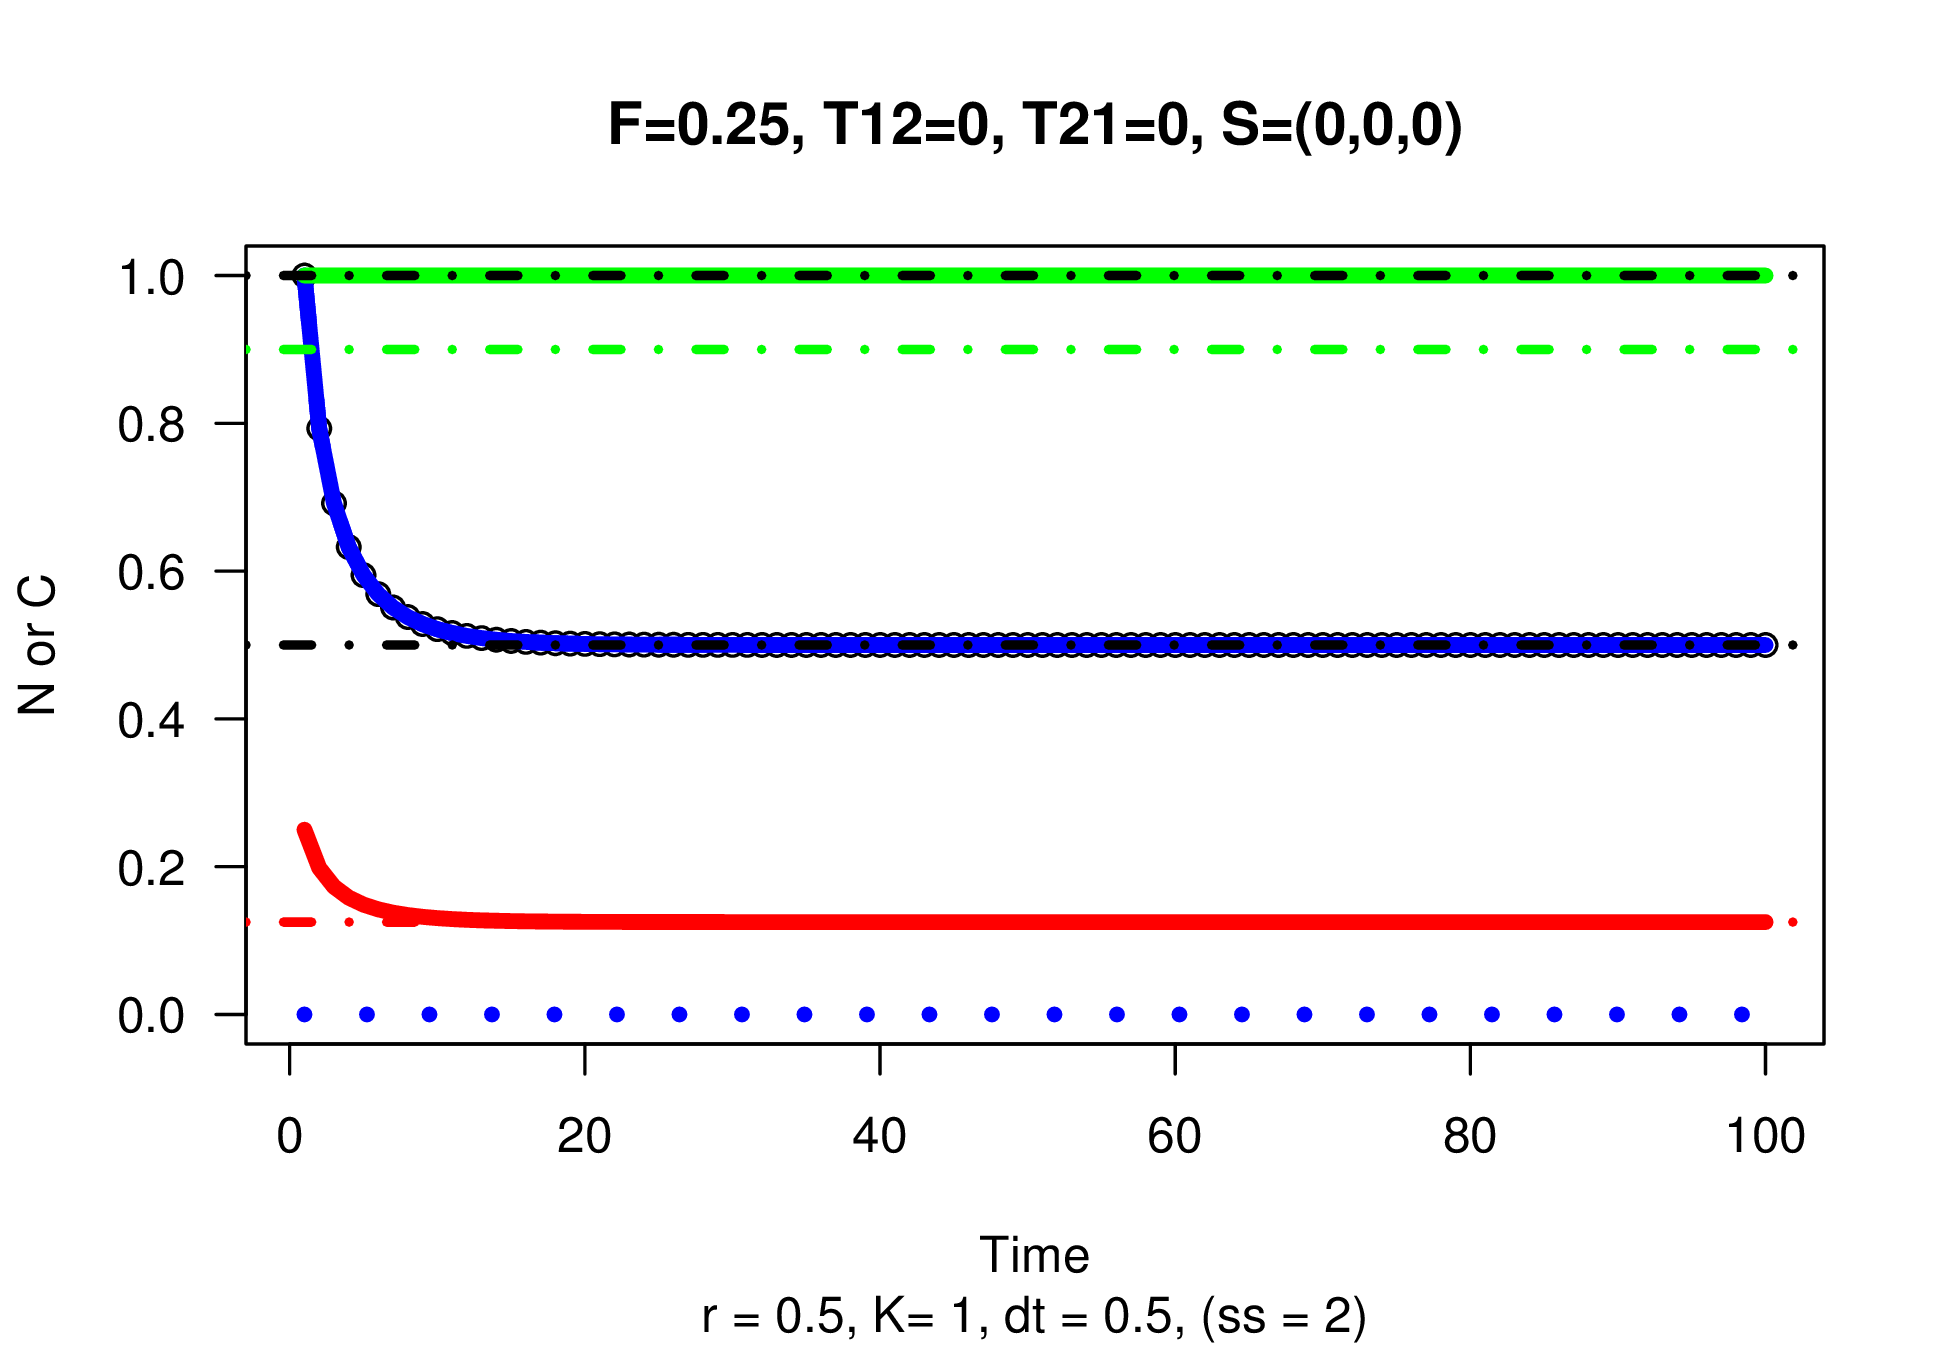
\includegraphics[height=0.8\textheight]{./graphics/r05F025T120T210S000.png}
\end{center}
\end{slide}


\begin{slide}\section{Emigration}
\begin{center}
Decrease total stock and catch; proportion local unchanged.
\begin{tabular}{cc}
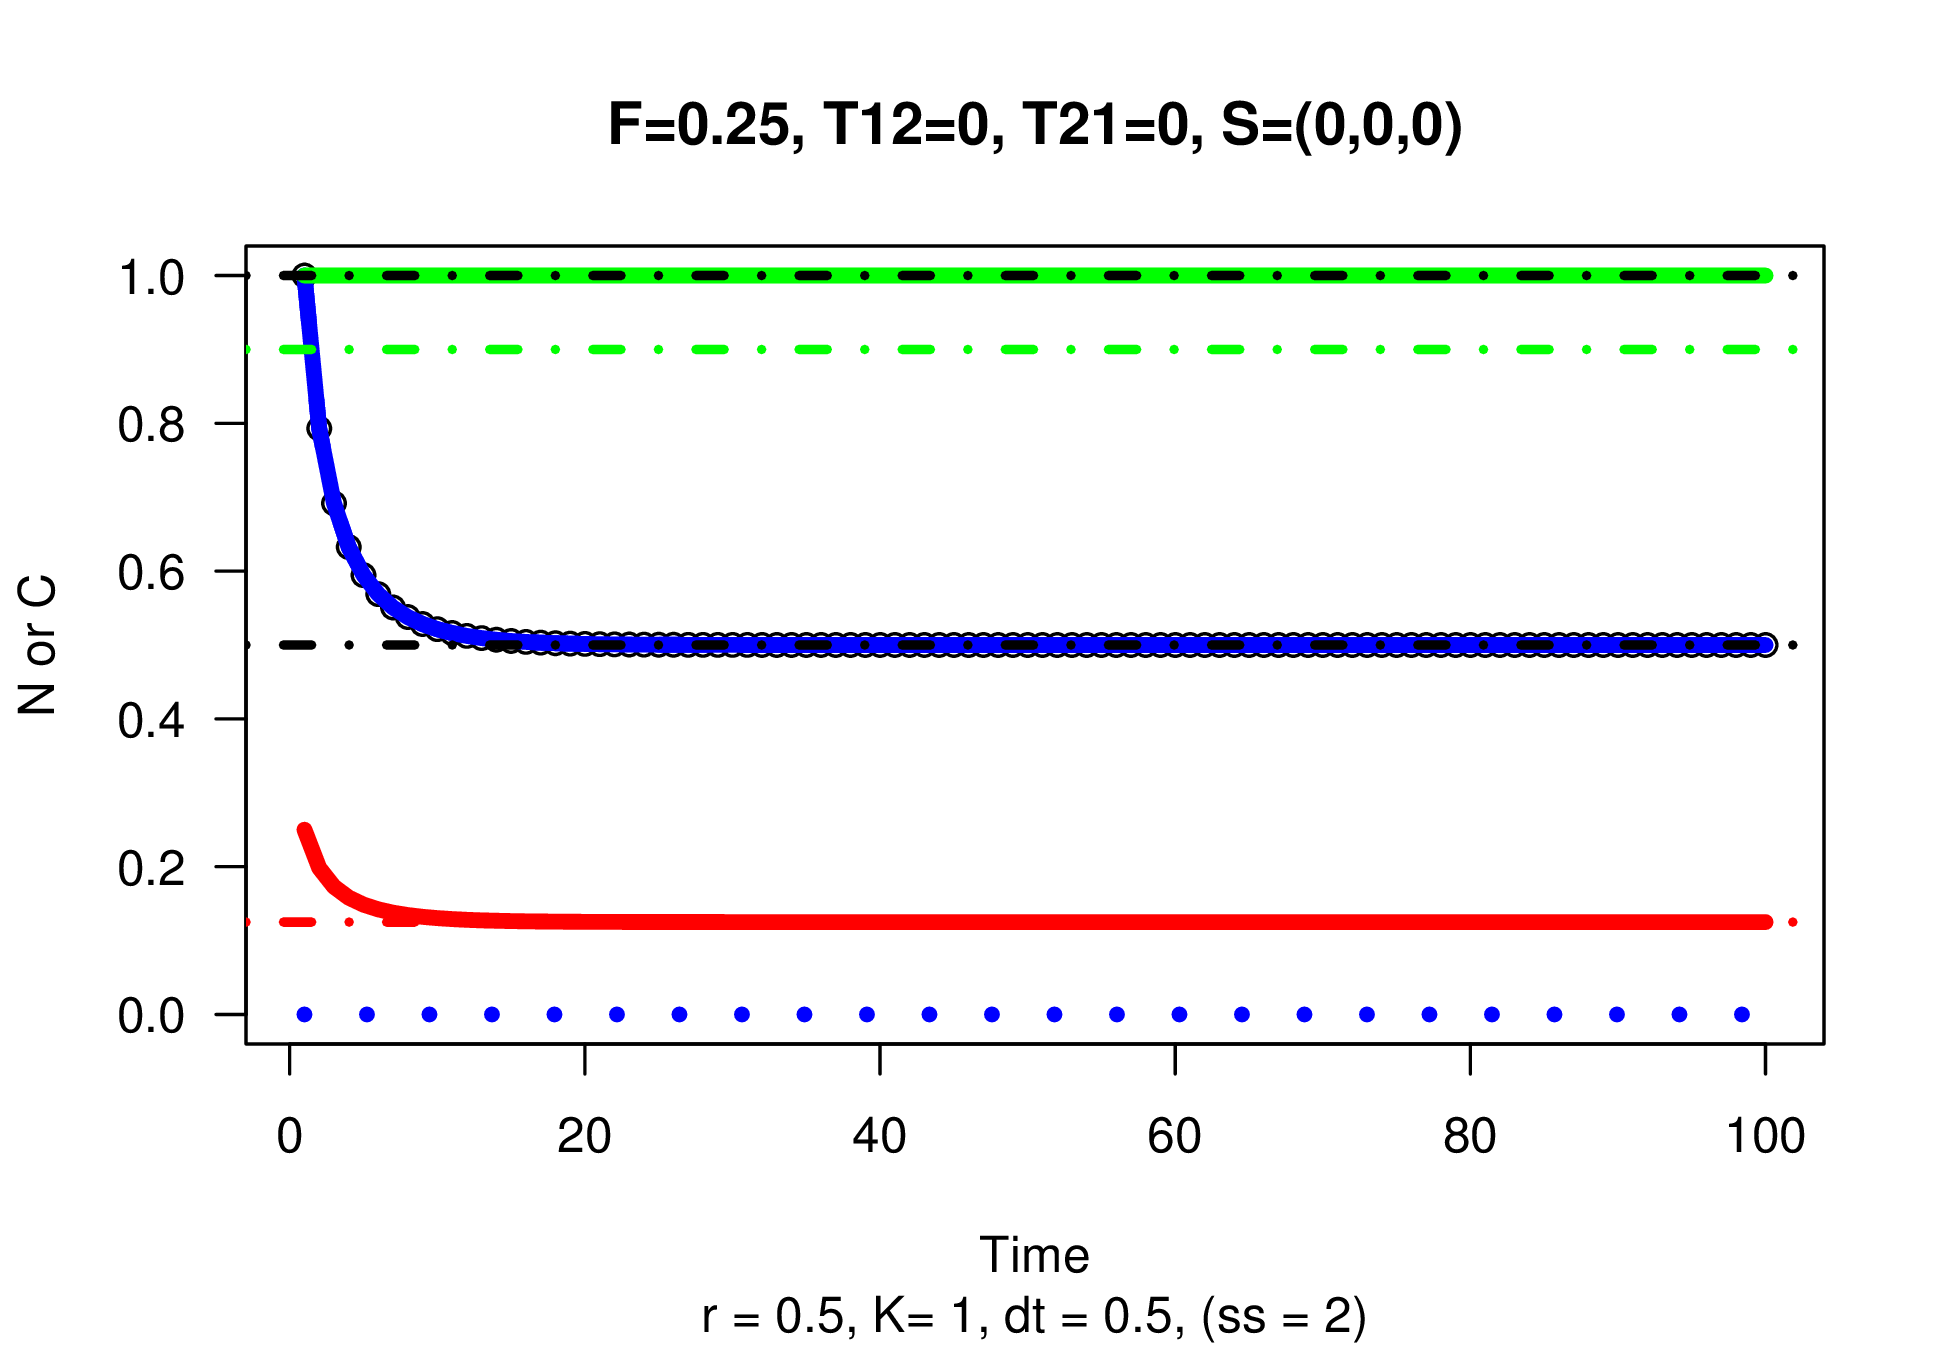
\includegraphics[height=0.35\textheight]{./graphics/r05F025T120T210S000.png}&
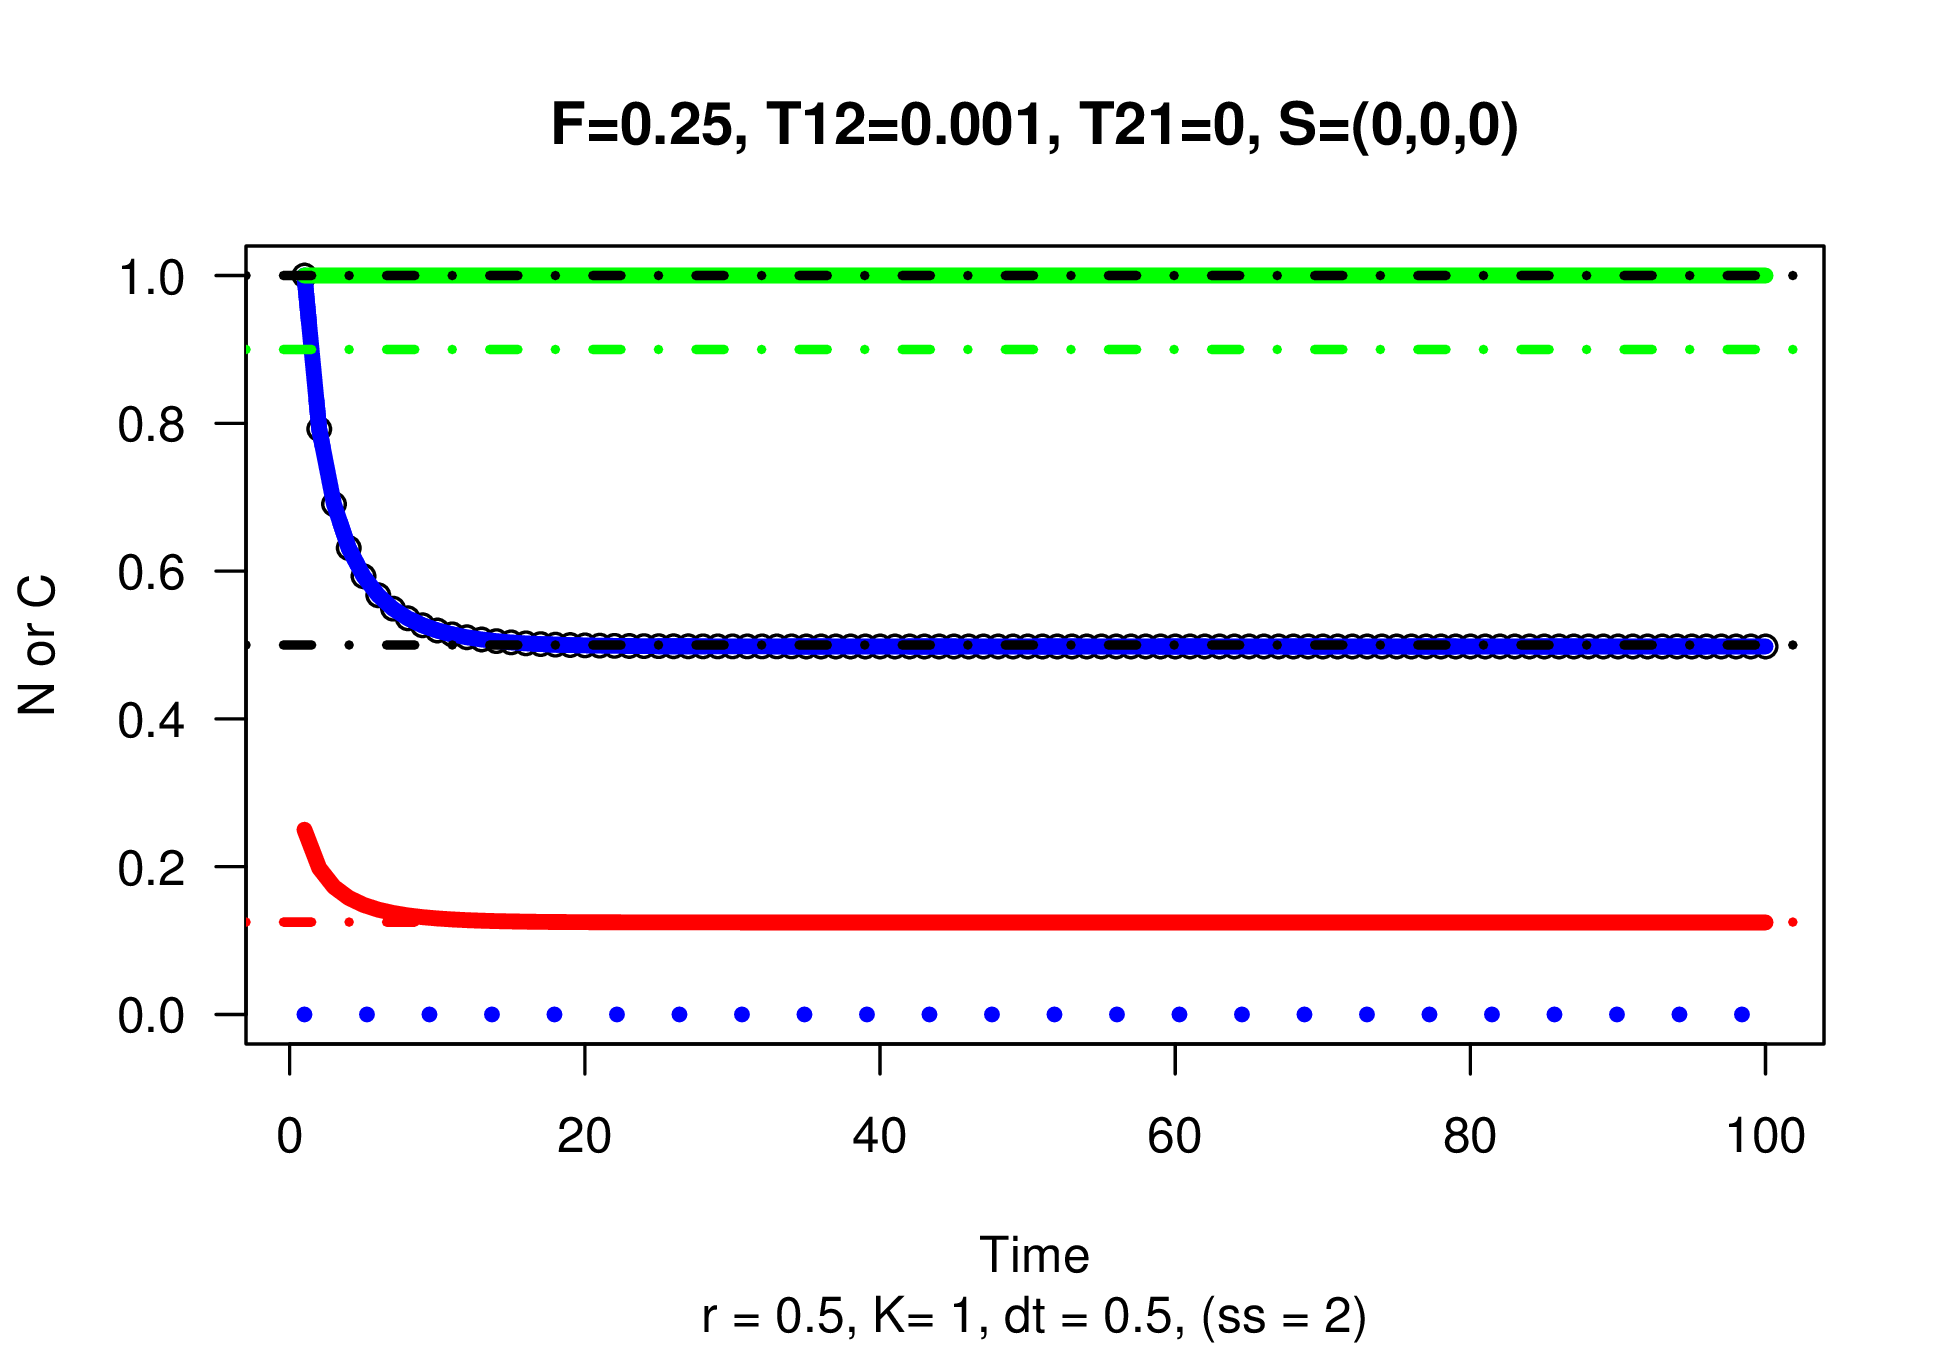
\includegraphics[height=0.35\textheight]{./graphics/r05F025T120001T210S000.png}\\
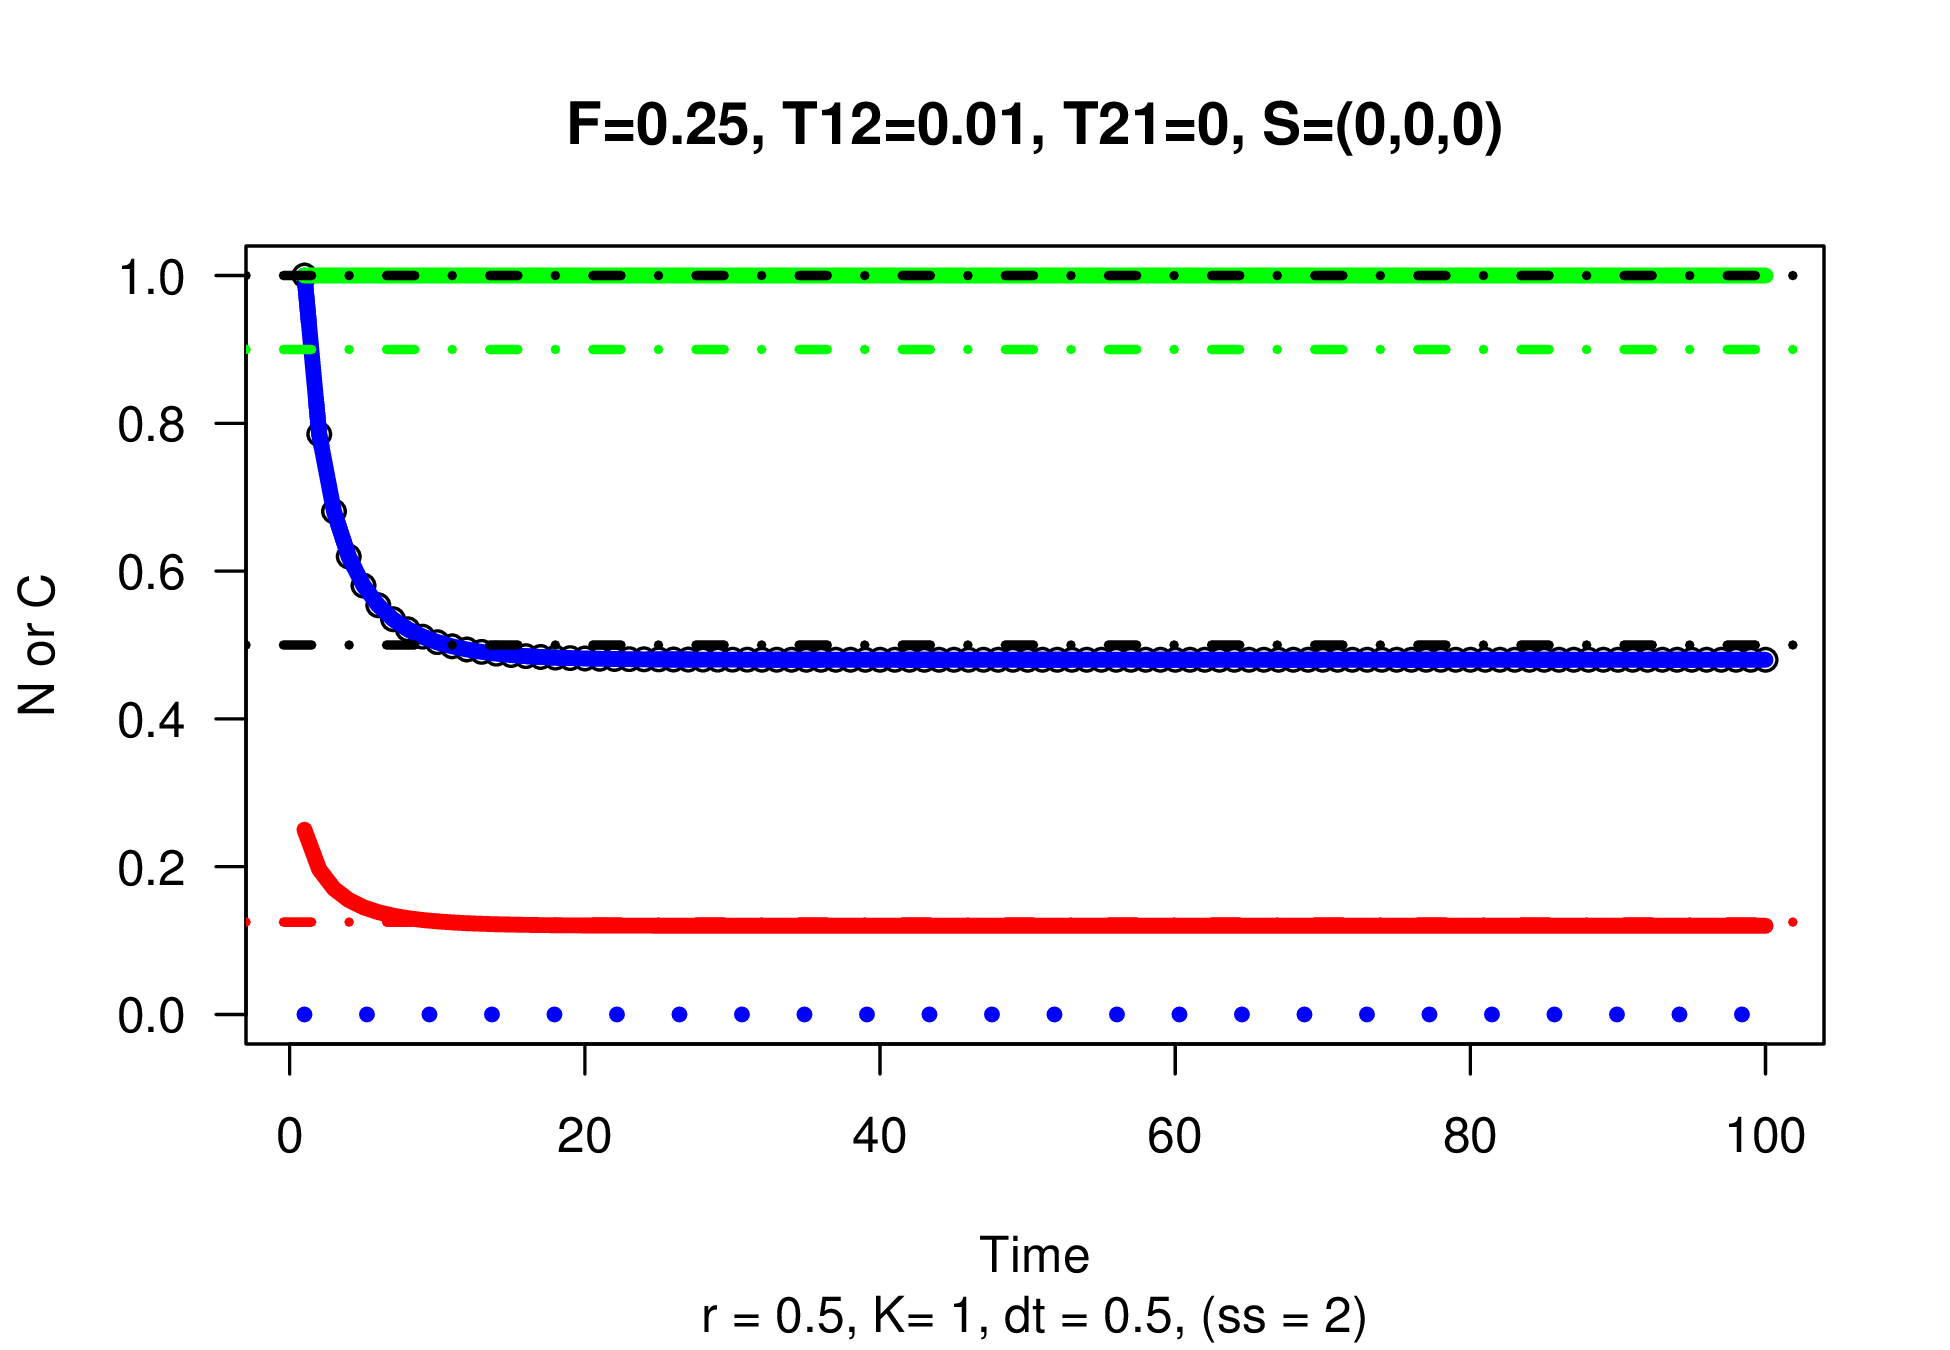
\includegraphics[height=0.35\textheight]{./graphics/r05F025T12001T210S000.png}&
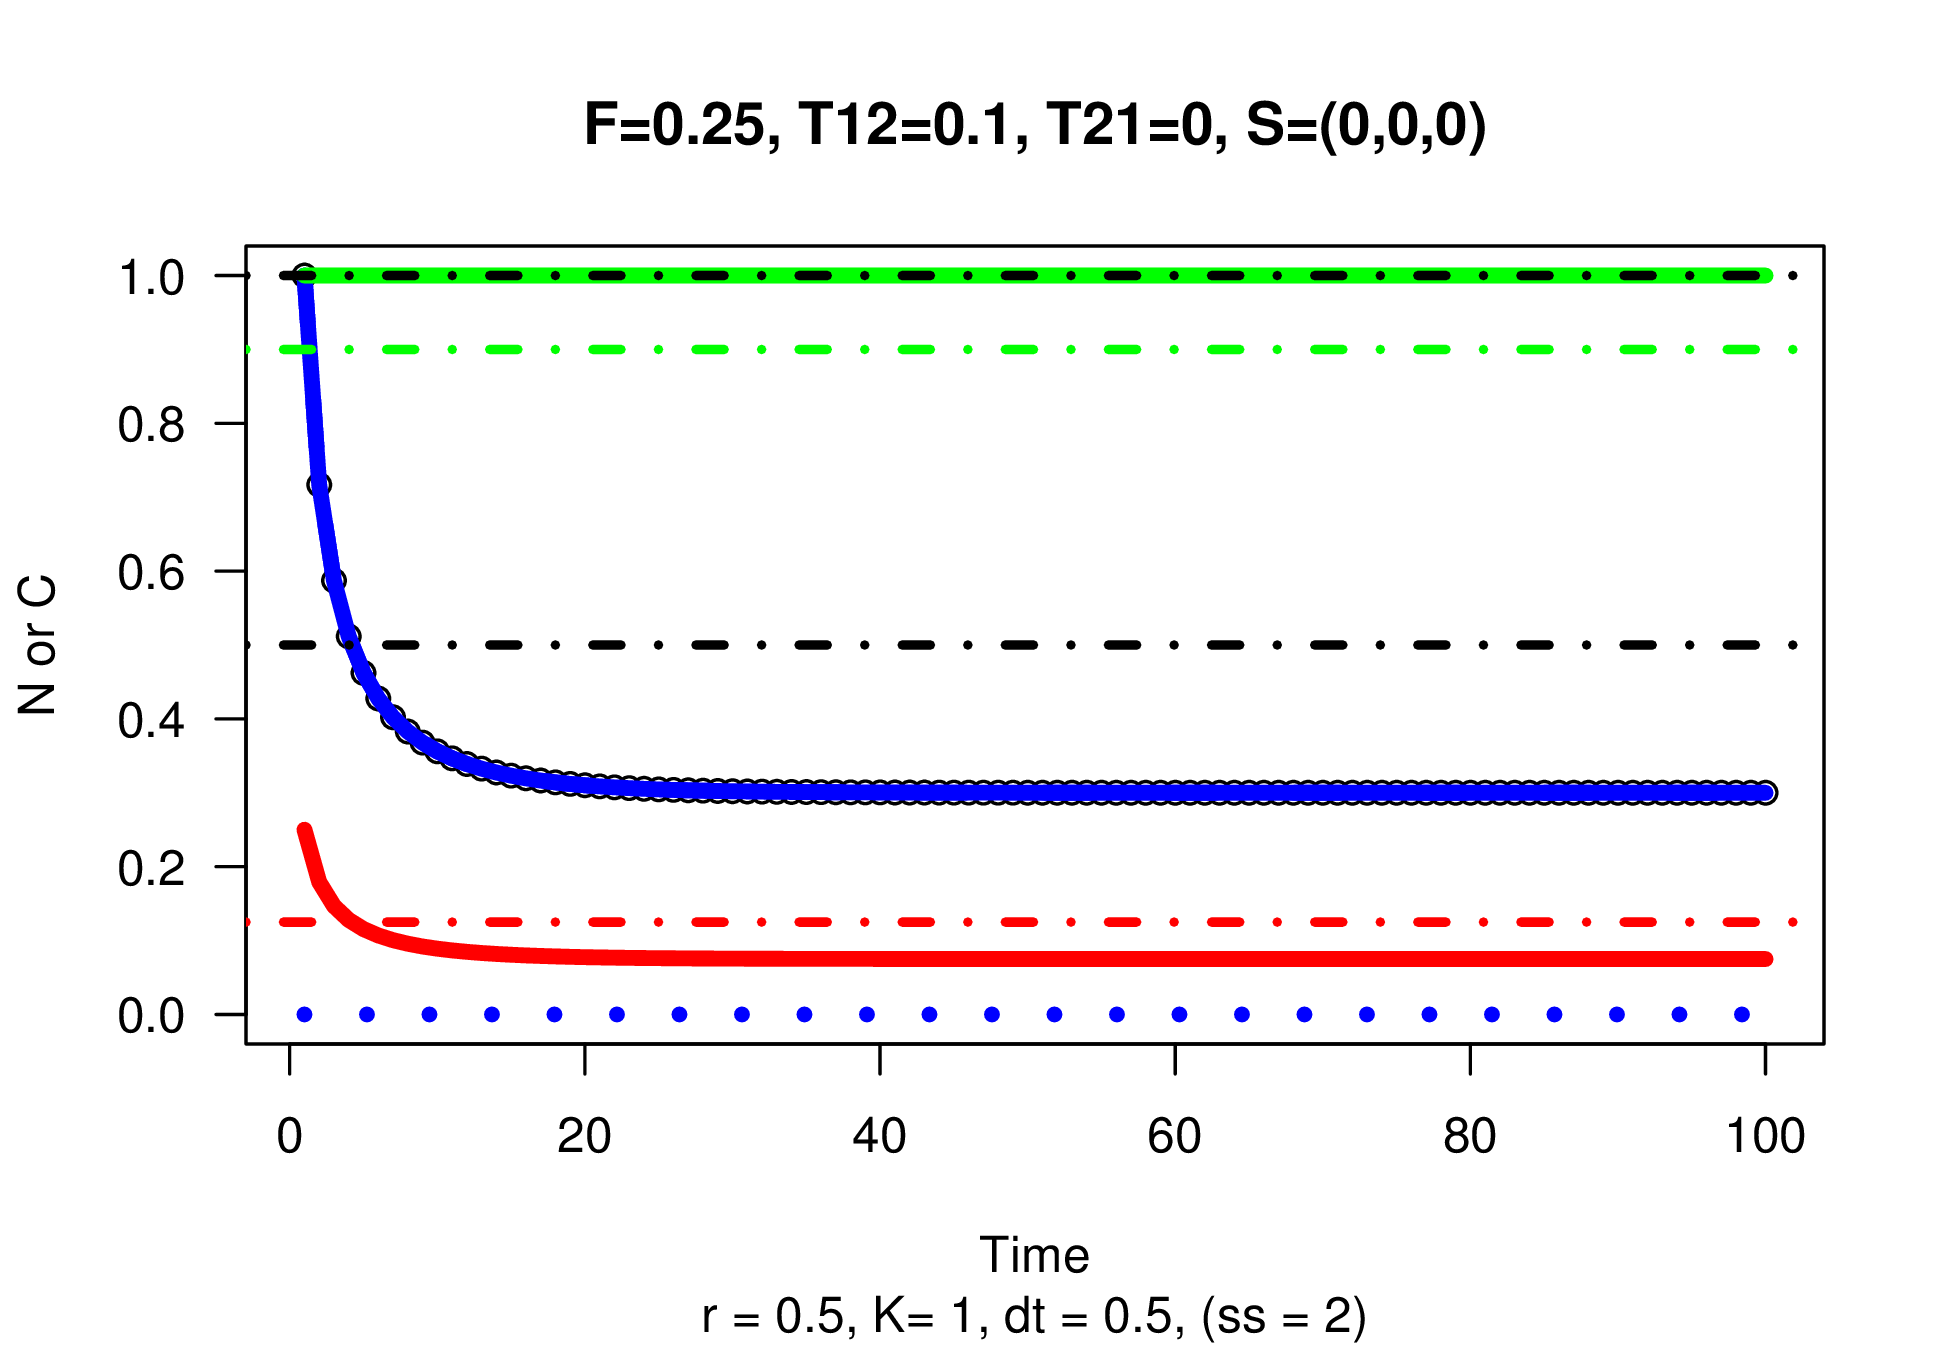
\includegraphics[height=0.35\textheight]{./graphics/r05F025T1201T210S000.png}\\
\end{tabular}
\end{center}
\end{slide}

\begin{slide}\section{Immigration}
\begin{center}
Increase total stock and catch; reduce proportion local.
\begin{tabular}{cc}
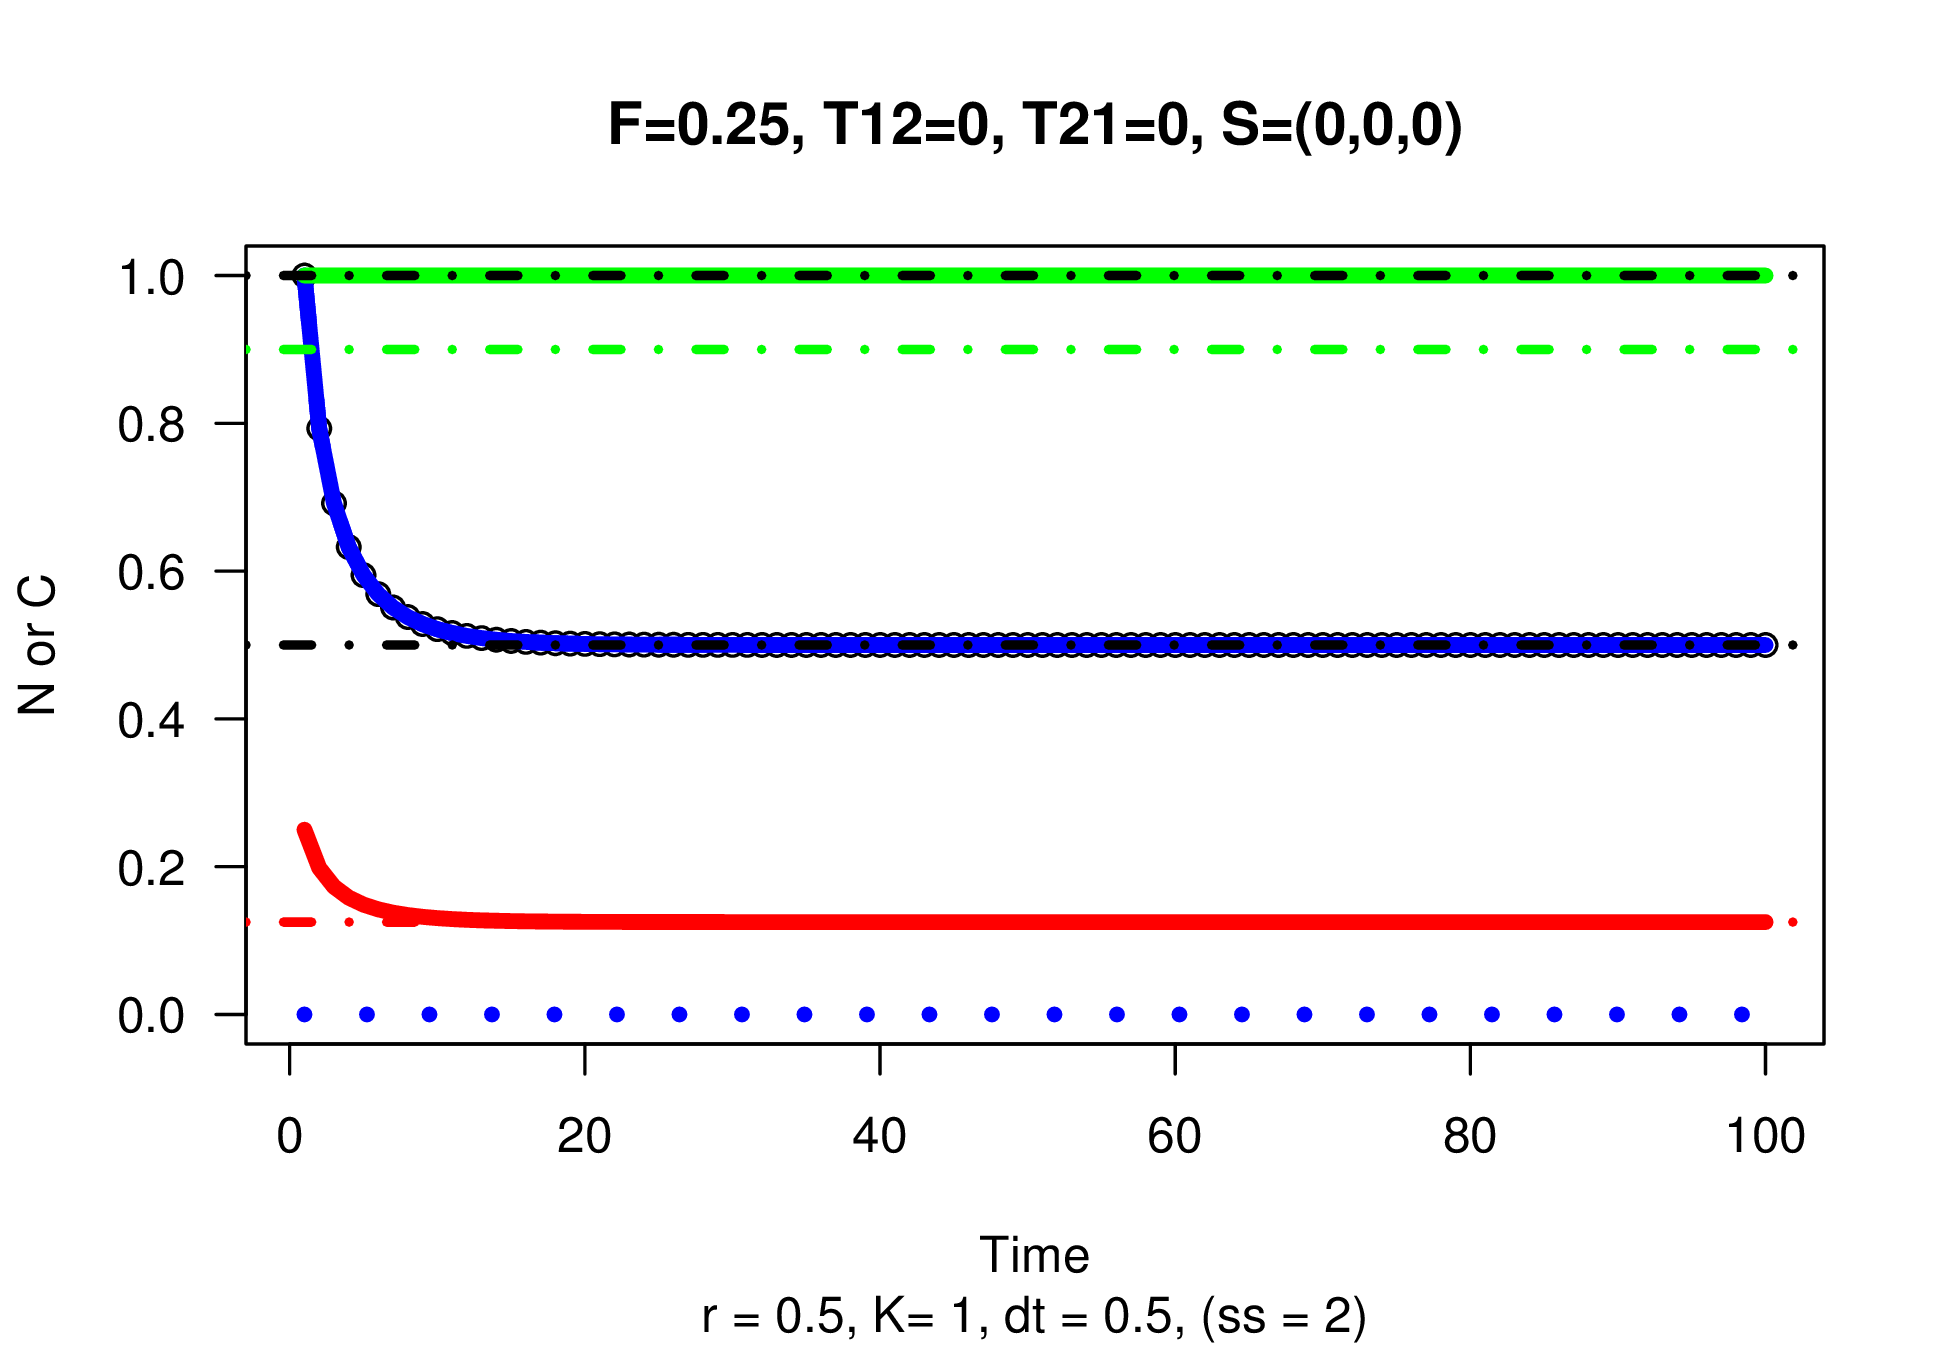
\includegraphics[height=0.35\textheight]{./graphics/r05F025T120T210S000.png}&
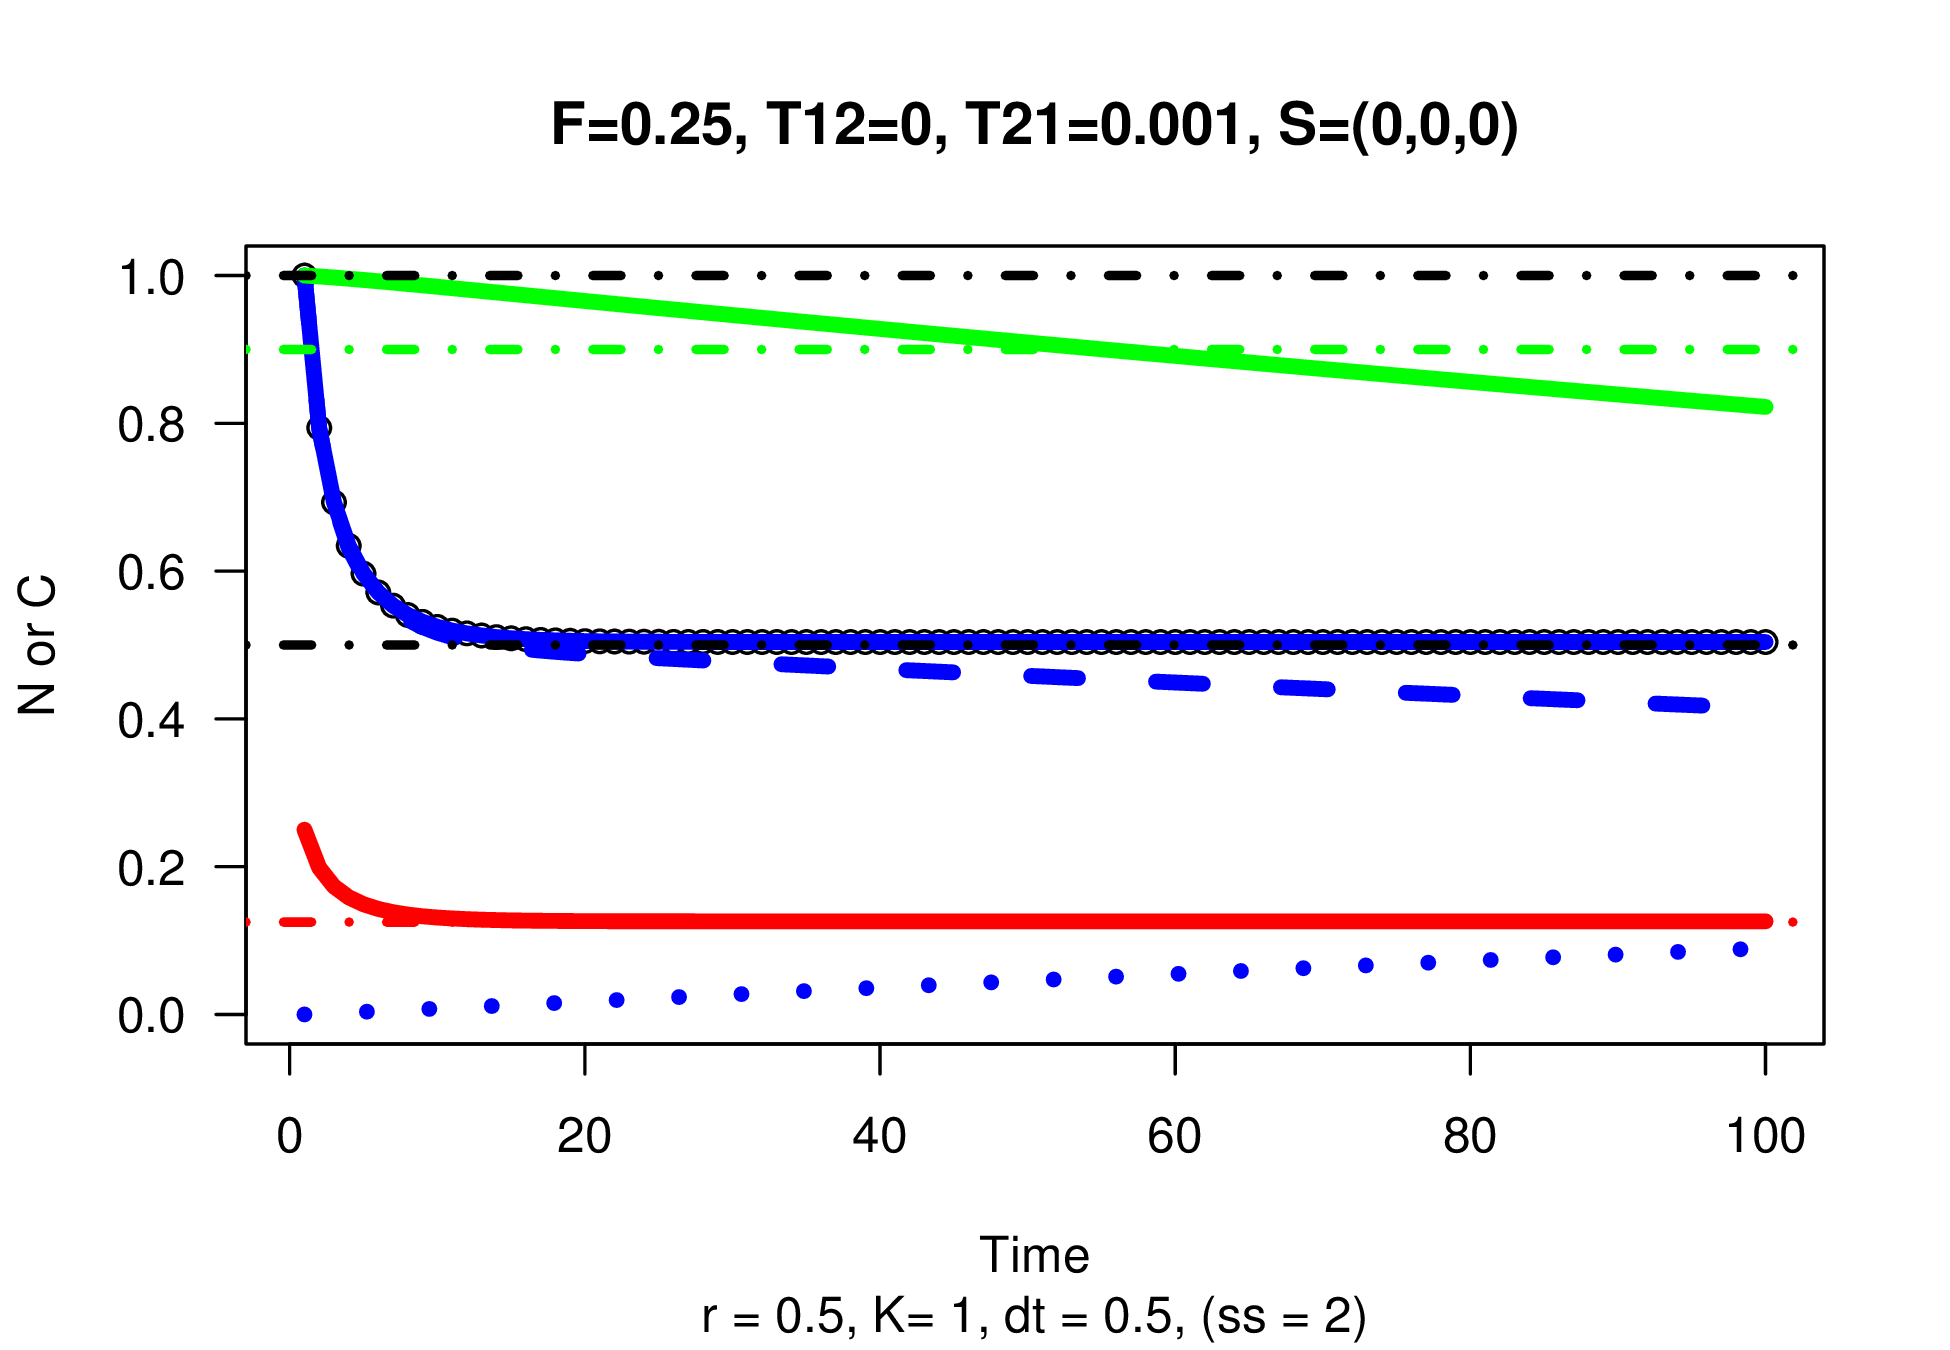
\includegraphics[height=0.35\textheight]{./graphics/r05F025T120T210001S000.png}\\
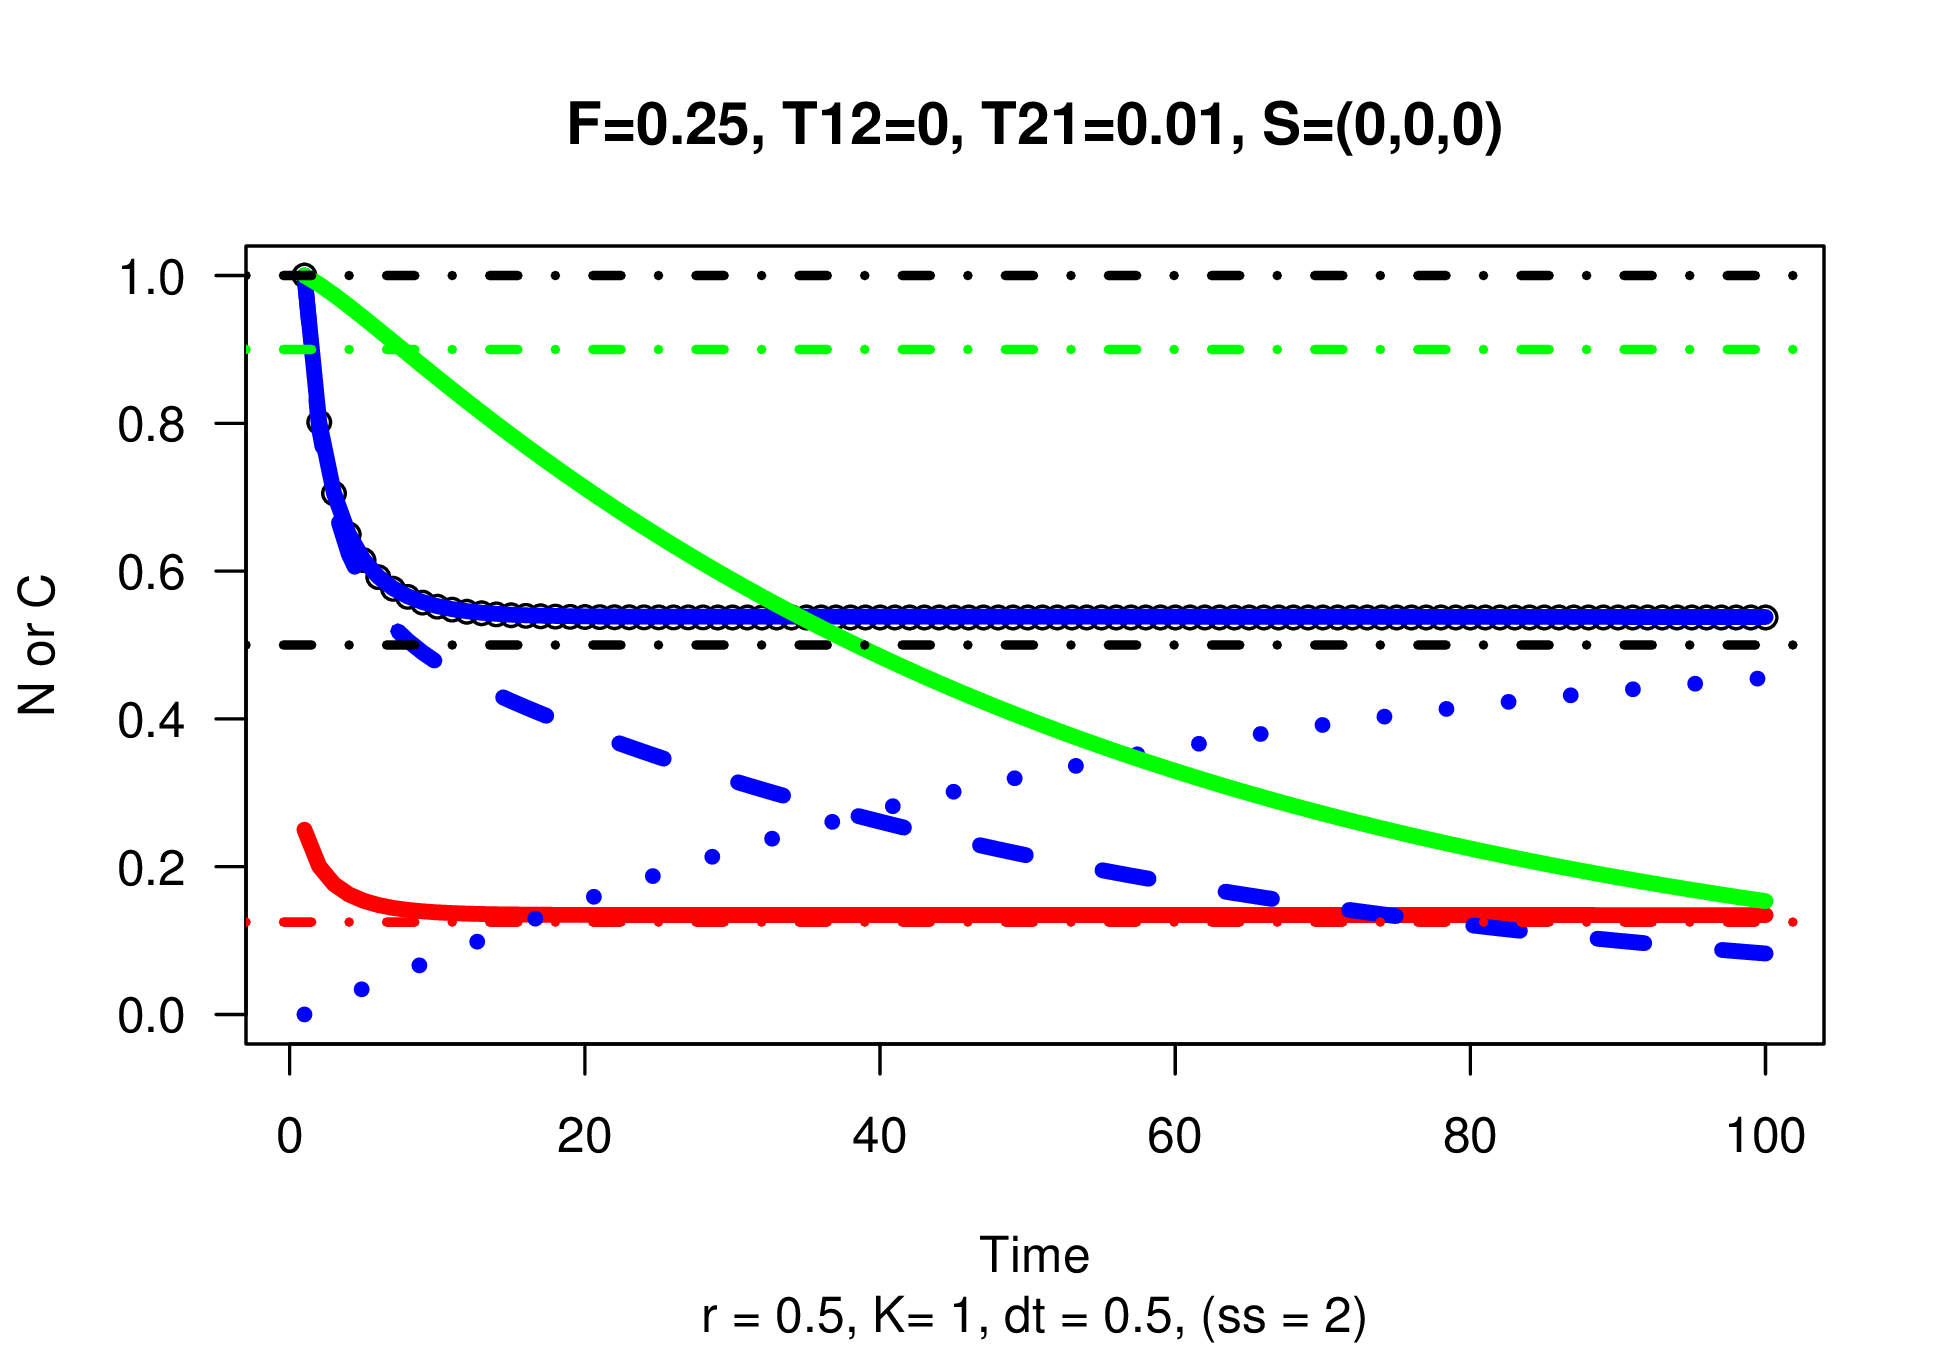
\includegraphics[height=0.35\textheight]{./graphics/r05F025T120T21001S000.png}&
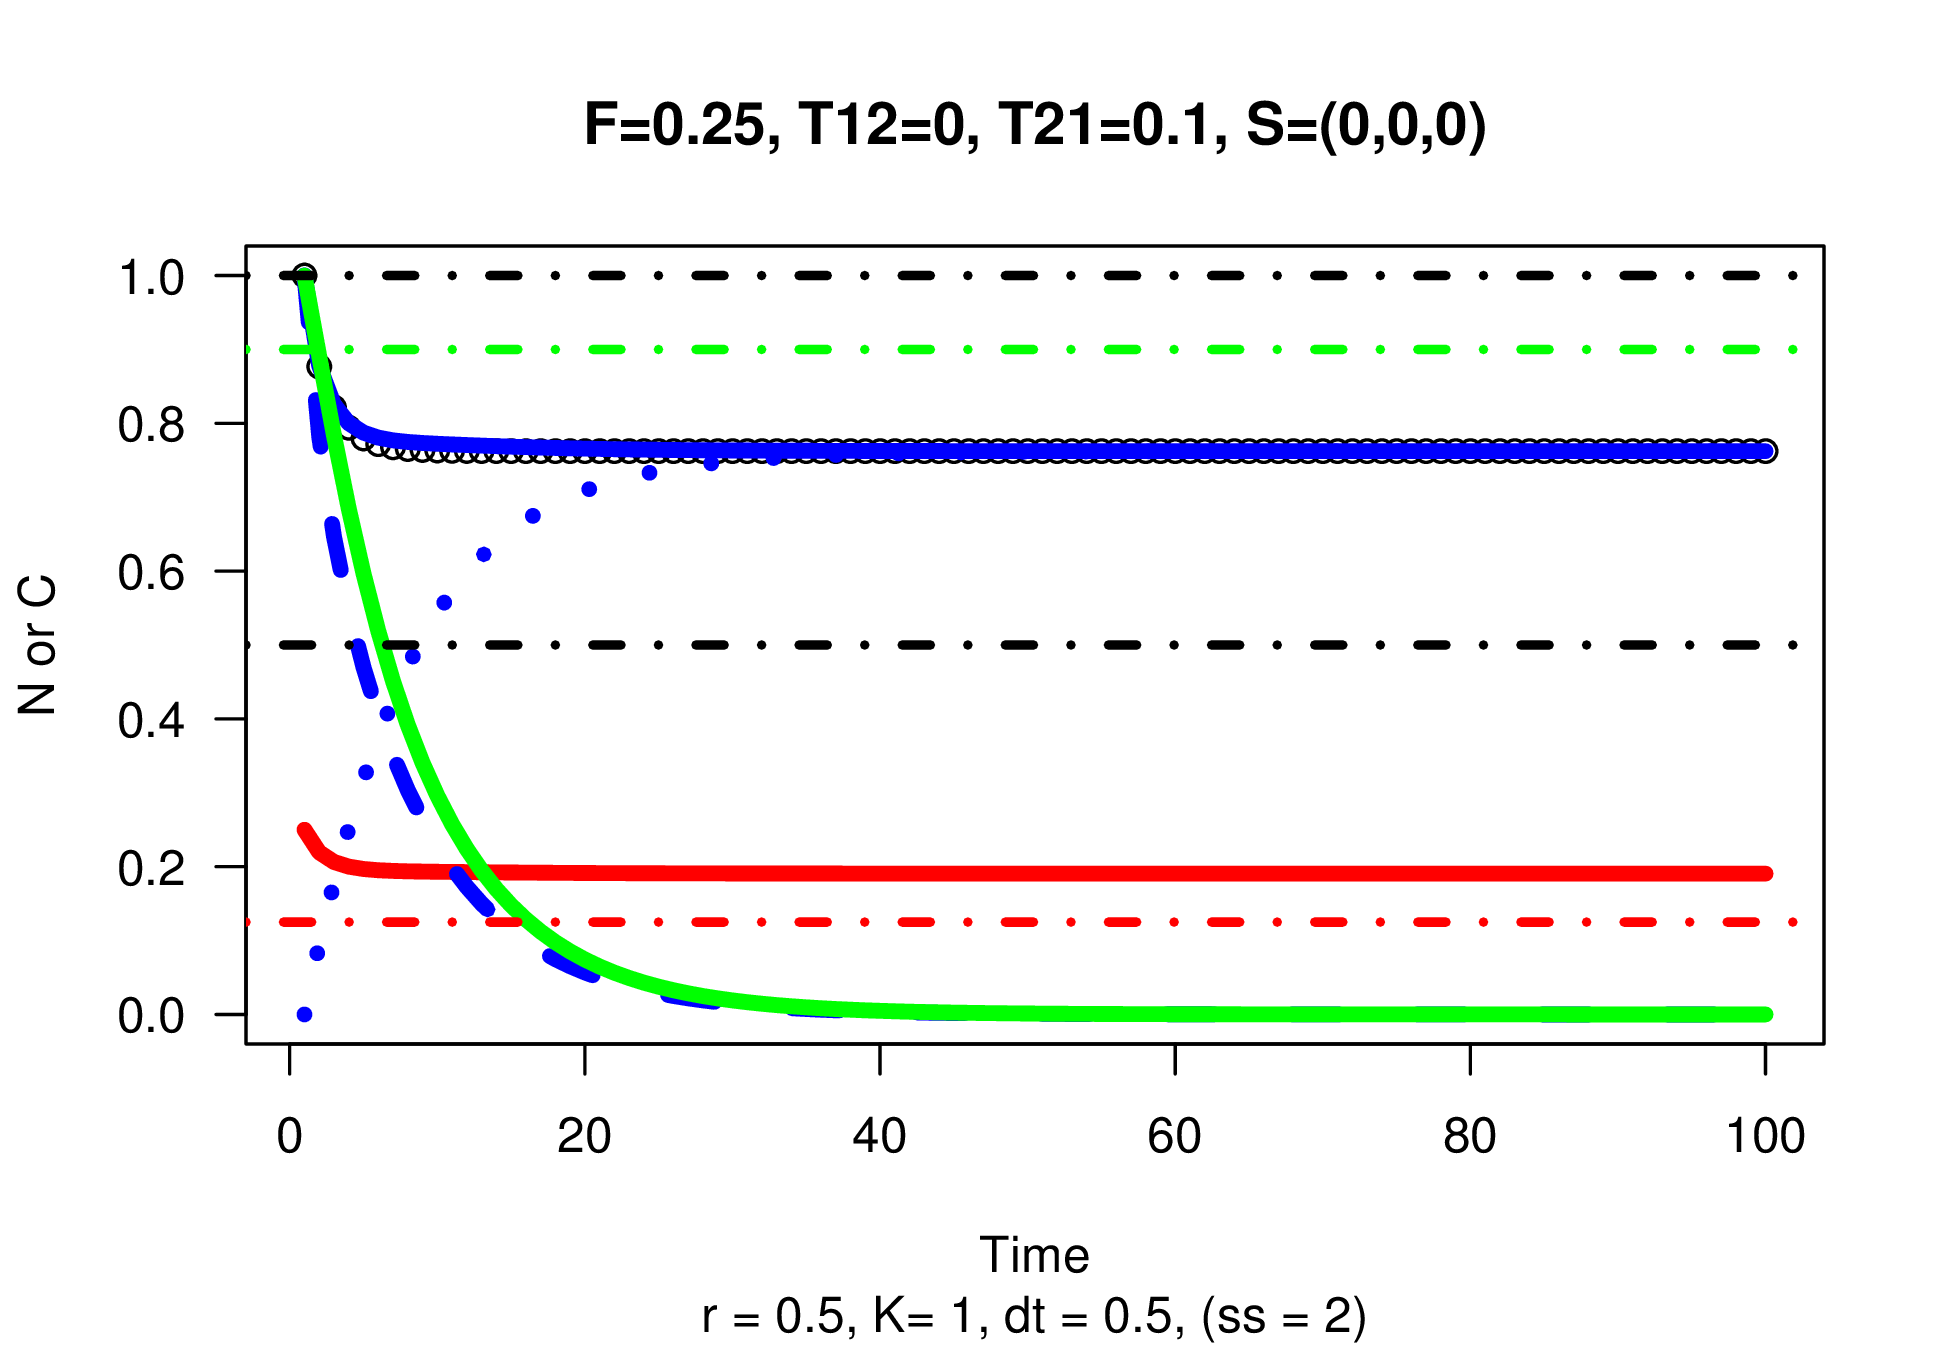
\includegraphics[height=0.35\textheight]{./graphics/r05F025T120T2101S000.png}\\
\end{tabular}
\end{center}
\end{slide}


\begin{slide}\section{Emigration, immigration and variability?}
\begin{center}
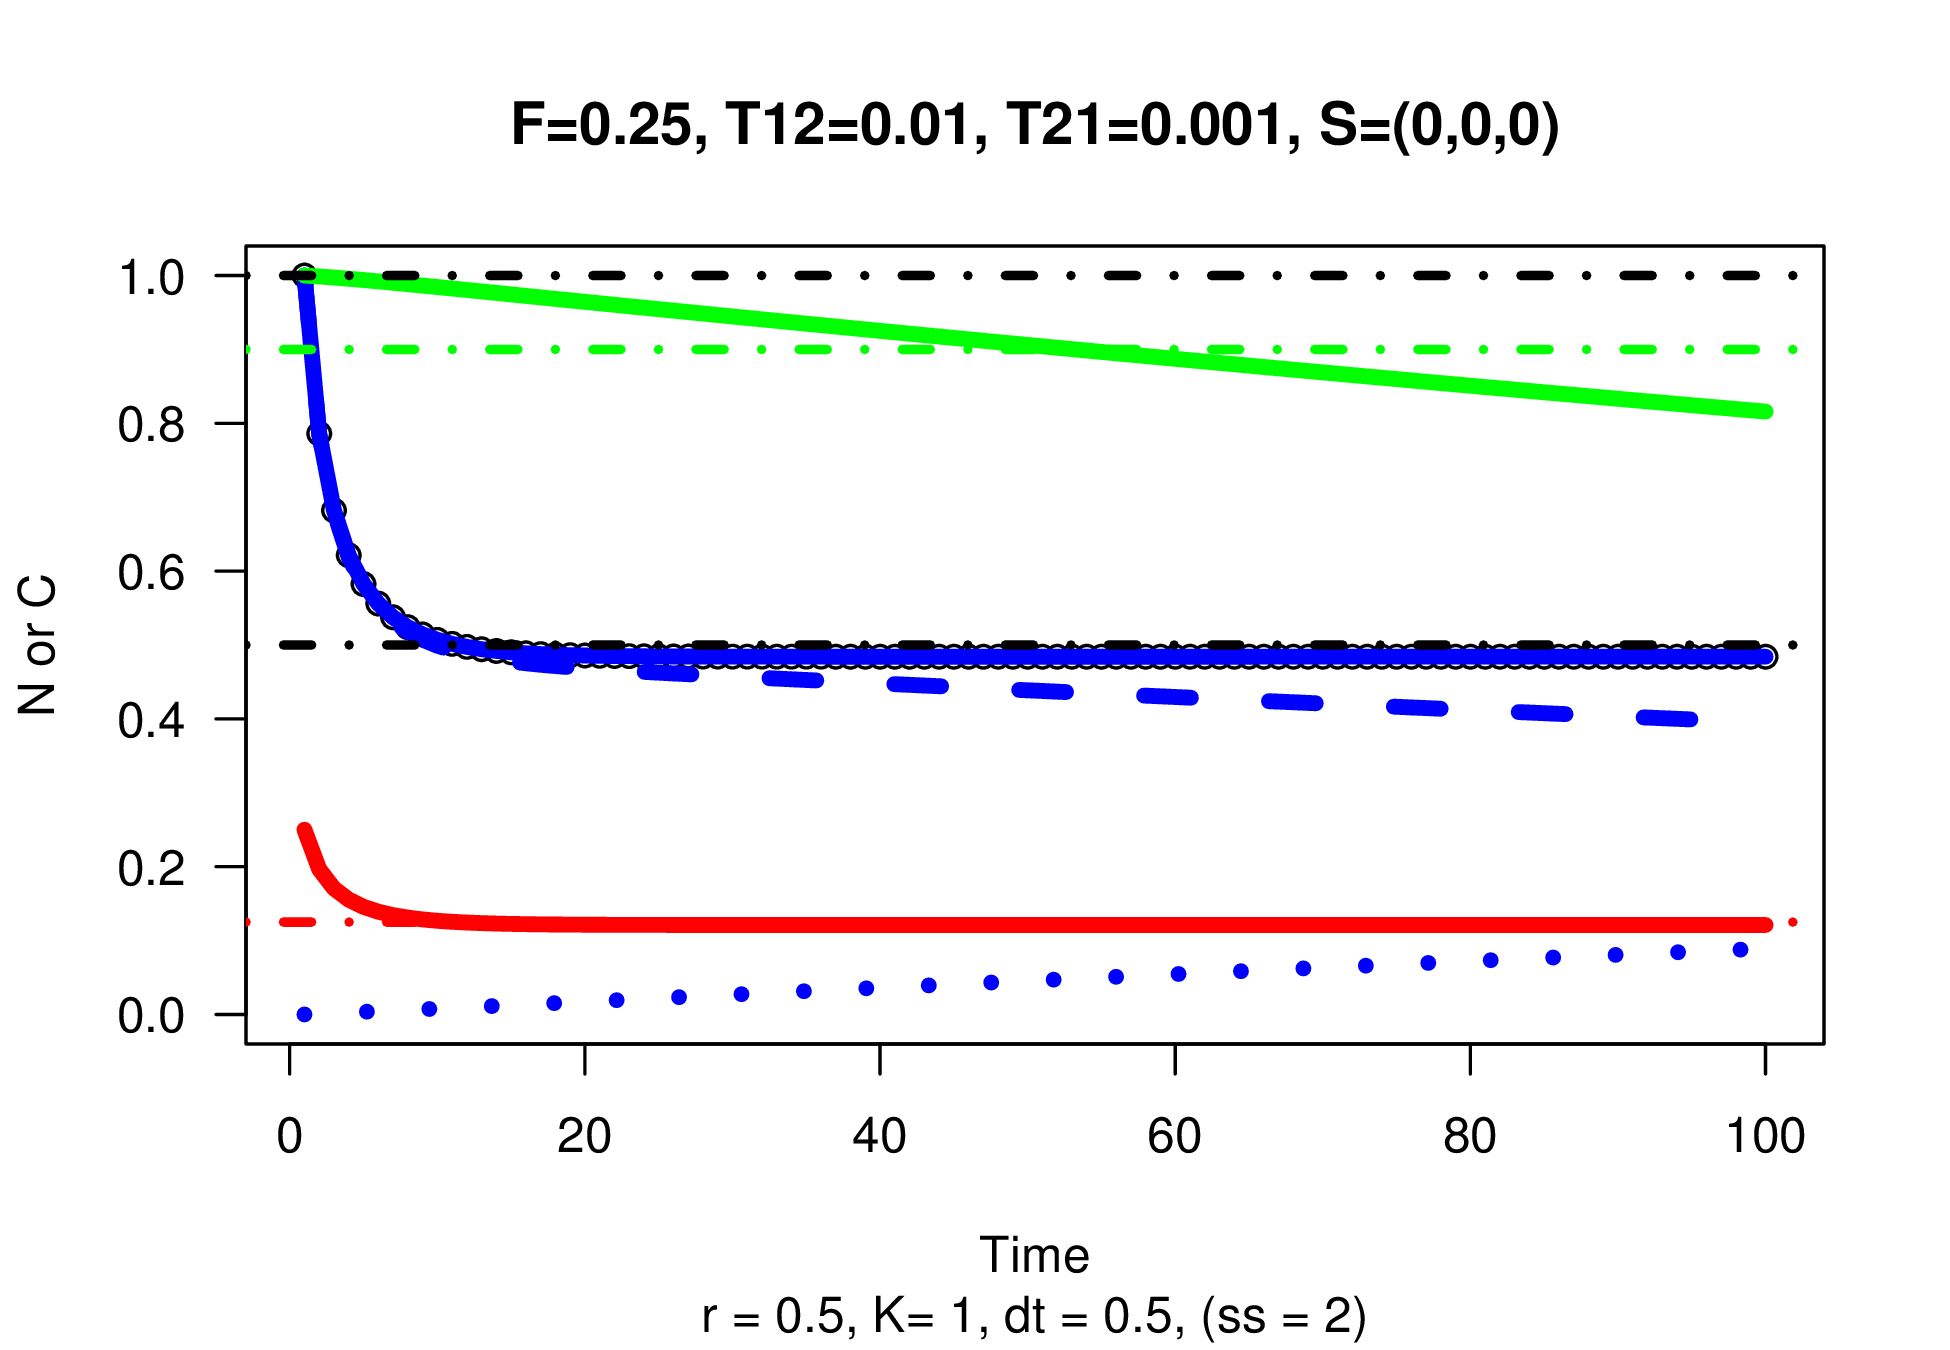
\includegraphics[height=0.35\textheight]{./graphics/r05F025T12001T210001S000.png}\\
Correlated log-normal random errors in $N_{11}$ and $N_{21}$\\
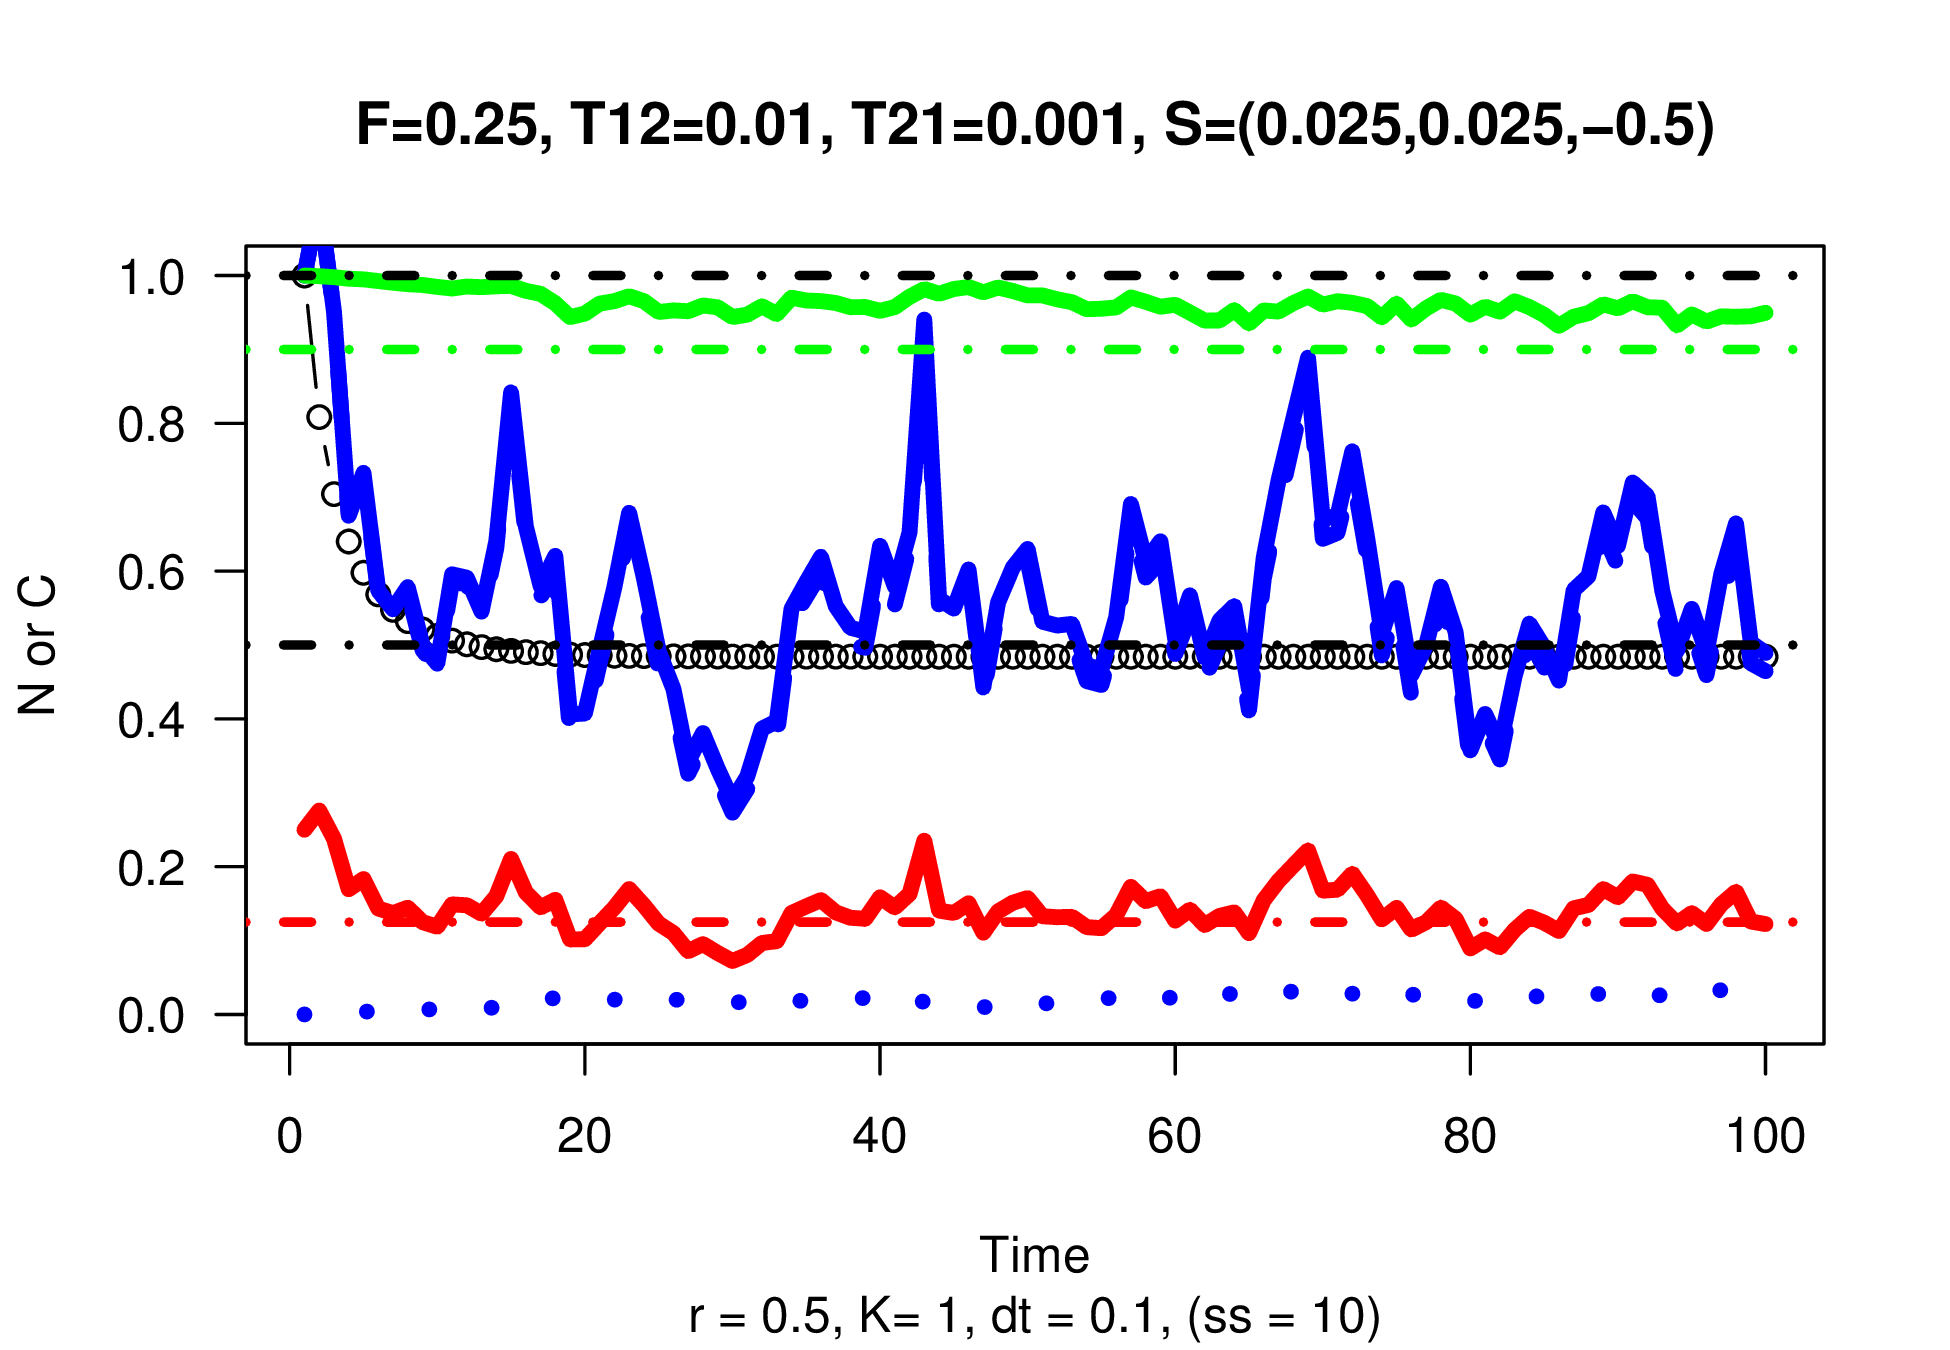
\includegraphics[height=0.35\textheight]{./graphics/r05F025T12001T210001S00250025-05.png}
\end{center}
\end{slide}

\begin{slide}\section{Next steps?}
\subsection{Is there a fishery management question here?}
\subsection{Implement state space model}
\begin{itemize}
\item Complete simulator (state equation) to include autocorrelated process error. 
\item Find and explore some data.
\item Write observation equation.
\item Test the model on simulated ``data''.
\item Estimate some parameters.
\end{itemize}
\end{slide}


\begin{slide}\section{Zzzzzz ... }
\begin{center}
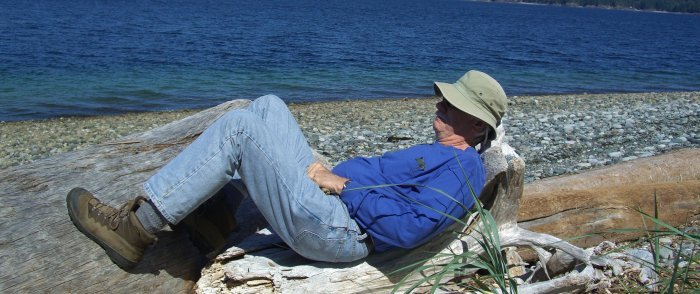
\includegraphics[width=0.8\textwidth]{./graphics/recumbant.png}
\end{center}
\end{slide}

\end{document}

